\documentclass[11pt,a4paper]{article}

\usepackage[a4paper,margin=1in]{geometry}
\usepackage{fontspec}
\usepackage{graphicx}
\usepackage{booktabs}
\usepackage{amsmath}
\usepackage[hypertexnames=false]{hyperref}
\usepackage{float}
\usepackage{xcolor}
\usepackage{url}
\usepackage[numbers]{natbib}
\usepackage{array}
\usepackage[font=small]{caption}

\setmainfont{Times New Roman}
\defaultfontfeatures{Ligatures=TeX}

\graphicspath{{figures/}}
\setlength{\parindent}{0pt}
\setlength{\parskip}{0.65em}
\urlstyle{same}
\captionsetup{labelfont=normalfont,textfont=normalfont,skip=4pt}

\begin{document}

\begin{center}
{\Large CDS540 Computer Vision Project Report\par}
\vspace{0.35cm}
{\LARGE Skin Lesion Classification with a Local Web Interface\par}
\vspace{0.25cm}
{\large Final Report\par}
\end{center}
\vspace{0.3cm}
\begin{flushleft}
{\normalsize
Student: Lai BAO, Shujian LIU, Zehan ZHAO, Liwen ZHENG, Junhao DU, Peng LIU\par
Tutor: Prof.\ Guo\par
Date: April 2026\par
}
\end{flushleft}
\vspace{0.6cm}

\begin{abstract}
This report presents a seven-class skin lesion classification system based on the HAM10000 dermoscopic image collection. The project combines grouped train--test preparation, a ResNet18 classifier with a squeeze-and-excitation style attention block, and a FastAPI interface for local inference. Images are reorganized from the metadata file into class folders, split by lesion identifier to reduce leakage, resized to \(224\times224\), normalized with ImageNet statistics, and augmented during training. The deployed interface supports upload, health checks, and local prediction history stored in SQLite. On the current grouped test set of 2{,}004 images, the provided model weights reach 0.92 accuracy, 0.87 macro F1, and 0.92 weighted F1. The report summarizes the system design, dataset preparation, exploratory analysis, evaluation results, and main limitations.
\end{abstract}

\section{Introduction}

Automatic analysis of dermoscopic images is an important problem in medical computer vision because early recognition of suspicious lesions can support screening and clinical review. The task remains challenging because several categories share similar colors, textures, and border patterns, while minority classes are much smaller than common benign categories \citep{esteva2017skin,tschandl2018ham10000}.

This project addresses the problem as an end-to-end system rather than an offline benchmark only. The current implementation uses HAM10000, prepares a grouped split by lesion identifier, applies a ResNet18-based classifier with channel attention, and exposes prediction through a FastAPI interface with local history. The report focuses on the implemented pipeline, the prepared dataset, the observed results, and the main remaining limitations.

\section{Project Objectives}

The main objective of this project is to build a complete seven-class skin lesion classification system and make it accessible through a local browser interface. The pipeline must reorganize HAM10000 into a grouped train--test split, preserve label consistency, reduce leakage across lesion identities, run a practical deep learning classifier, and report class-aware evaluation results.

A second objective is to connect model performance with usable inference. The deployed system should return a clear top prediction and confidence score for an uploaded dermoscopic image and keep previous results available through local history. The project is centered on single-image classification and does not target segmentation, detection, or cloud deployment.

\section{System Design and Architecture}

The project is organized as an end-to-end system rather than a standalone training notebook. Original HAM10000 images and metadata are reorganized into grouped training and testing folders by \texttt{prepare\_data.py}. Offline training and evaluation are handled by \texttt{main.py}, while \texttt{app.py} loads the saved weight file for local inference and serves the browser interface, prediction endpoint, health check, and history API.

\begin{figure}[H]
    \centering
    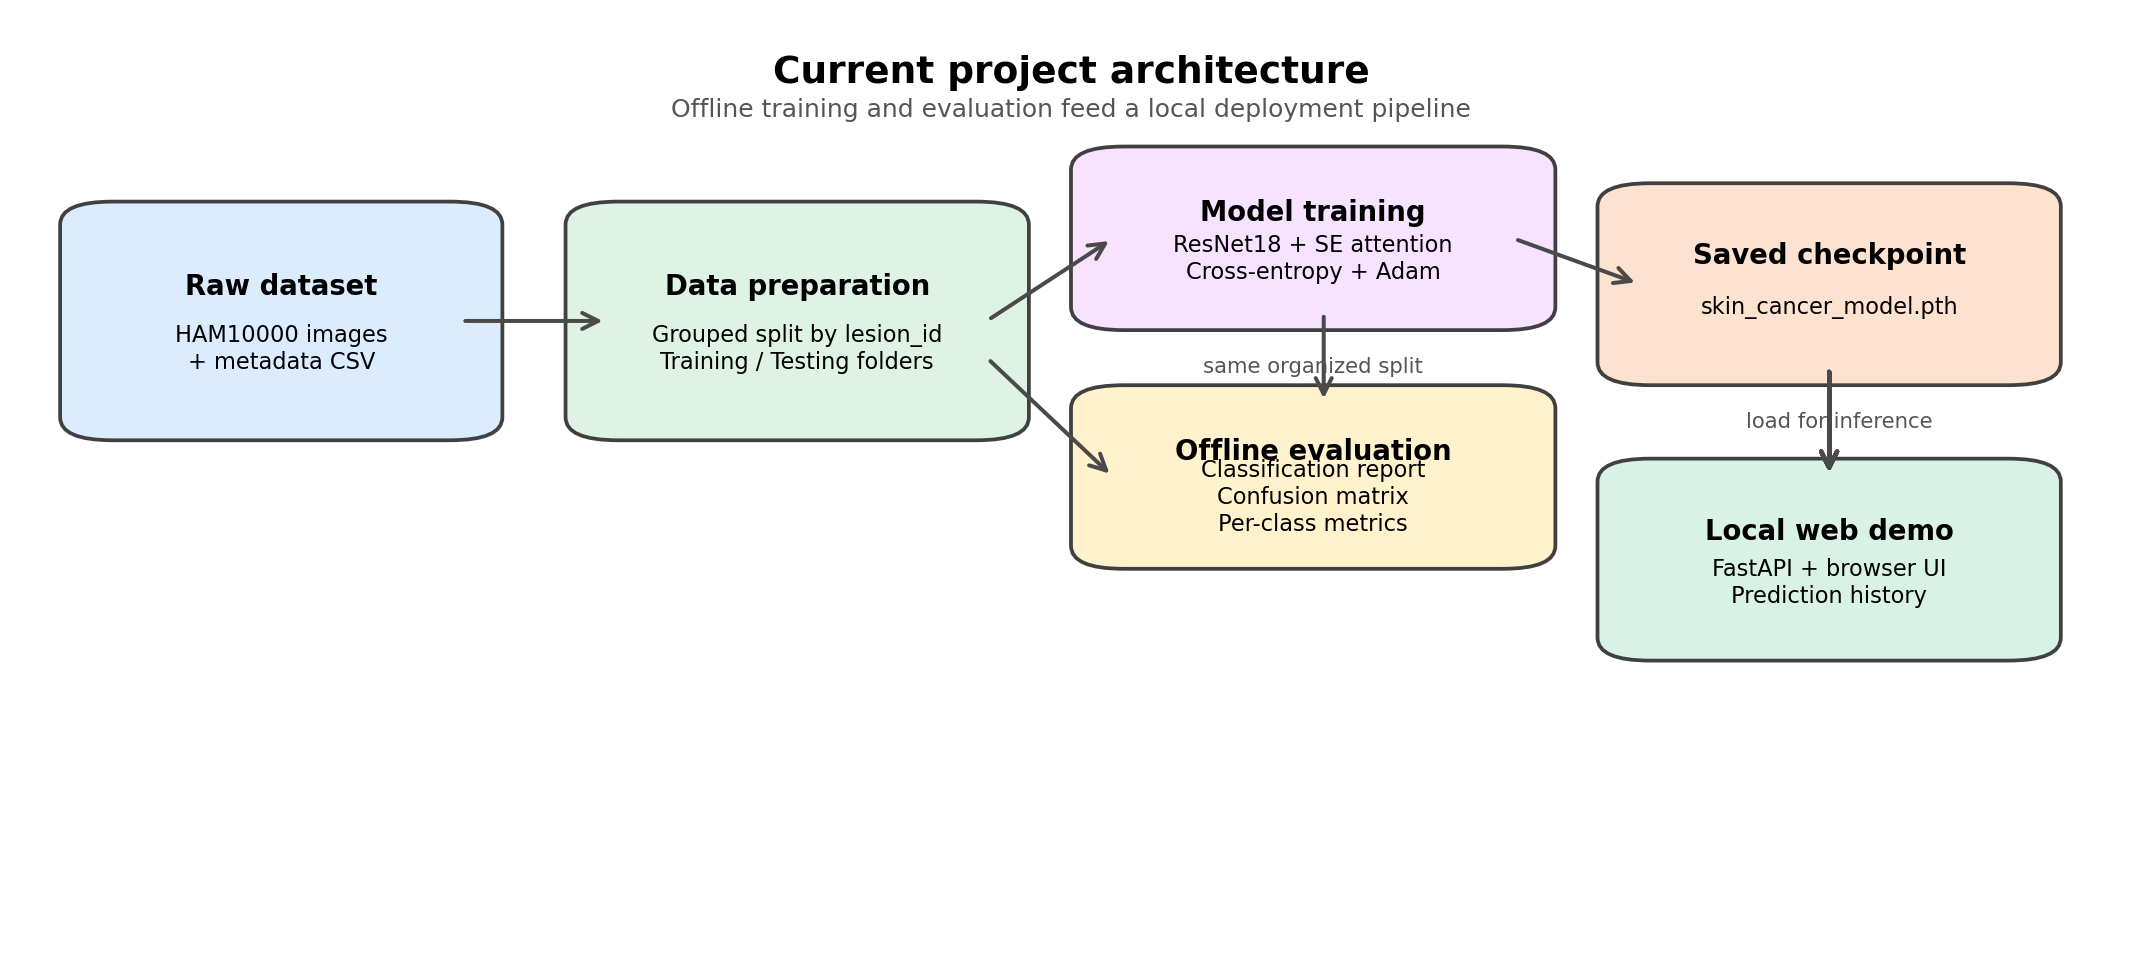
\includegraphics[width=0.95\textwidth]{system_architecture.png}
    \caption{Project workflow for data preparation, model inference, and local history storage.}
    \label{fig:architecture}
\end{figure}

Figure~\ref{fig:architecture} summarizes the workflow. The offline branch prepares the grouped split, trains the classifier, and saves the checkpoint. The online branch reuses that checkpoint in FastAPI, returns predictions to the browser, and stores recent outputs in SQLite.

\section{Algorithm and Implementation Details}

The project uses a ResNet18 image classifier \citep{he2016resnet} with a squeeze-and-excitation style channel attention block \citep{hu2018senet}. Training uses pretrained torchvision weights and a task-specific seven-class head. The implementation is written in PyTorch \citep{paszke2019pytorch} for single-image dermoscopic classification.

\begin{table}[H]
    \centering
    \caption{Current algorithm summary.}
    \label{tab:algorithm}
    \begin{tabular}{>{\raggedright\arraybackslash}p{0.28\textwidth} >{\raggedright\arraybackslash}p{0.62\textwidth}}
        \toprule
        Component & Current implementation \\
        \midrule
        Task type & Seven-class classification \\
        Input & One RGB dermoscopic image \\
        Backbone & ResNet18 \\
        Training strategy & Transfer learning \\
        Attention module & SE-style channel attention \\
        Classifier head & 512$\rightarrow$256$\rightarrow$7 with ReLU and Dropout(0.4) \\
        Image preprocessing & Resize \(224\times224\), tensor, ImageNet normalization \\
        Training augmentation & H/V flips, 20$^\circ$ rotation, mild color jitter \\
        Loss function & Cross-entropy \\
        Optimizer & Adam \\
        Learning-rate schedule & Cosine annealing, minimum \(10^{-6}\) \\
        Batch size and epochs & 32, 30 \\
        Inference rule & Top-1 softmax with confidence \\
        Extra deployment logic & Blank-image heuristic, threshold 0.5 \\
        Main strength & Compact and deployable \\
        Main limitation & No validation stage, class imbalance \\
        \bottomrule
    \end{tabular}
\end{table}

This design balances standard transfer learning with lightweight deployment. Its main limits are unchanged: the model predicts one label per image, does not localize lesions, and returns confidence scores that are not formally calibrated.

\section{Dataset Description, Cleaning, and Exploratory Analysis}

The project uses the HAM10000 dermoscopic image collection \citep{tschandl2018ham10000}. The active pipeline reads the original image archive and \texttt{HAM10000\_metadata.csv}, reorganizes images into class folders, and loads them through \texttt{ImageFolder}. The alternative low-resolution CSV representations stored in the archive are not used by the current code.

\begin{table}[H]
    \centering
    \caption{Dataset summary from the current repository.}
    \label{tab:datasetsummary}
    \begin{tabular}{>{\raggedright\arraybackslash}p{0.30\textwidth} >{\raggedright\arraybackslash}p{0.60\textwidth}}
        \toprule
        Item & Current dataset evidence \\
        \midrule
        Source dataset & HAM10000 \\
        Original inputs & Two image folders and one metadata CSV \\
        Active label field & \texttt{dx} \\
        Final organization & \texttt{archive/Training} and \texttt{archive/Testing} class folders \\
        Split method & Grouped by \texttt{lesion\_id}, stratified by \texttt{dx} \\
        Training images & 8{,}011 \\
        Testing images & 2{,}004 \\
        Training lesions & 5{,}975 unique lesions \\
        Testing lesions & 1{,}495 unique lesions \\
        Leakage check & 0 image overlap, 0 lesion overlap \\
        Original image size & \(600\times450\) \\
        Metadata used & \texttt{lesion\_id}, \texttt{image\_id}, \texttt{dx}, \texttt{dx\_type}, \texttt{age}, \texttt{sex}, \texttt{localization} \\
        \bottomrule
    \end{tabular}
\end{table}

The preparation script performs practical cleaning and reorganization rather than deep manual curation. It validates the input paths, reads the metadata file, builds a grouped split, recreates the output directories, and copies images into diagnosis-specific folders. Based on the available code and regenerated statistics, the current pipeline removes lesion-level leakage and aligns folder names with metadata labels. No explicit evidence of corrupted-image filtering, manual relabeling, or duplicate removal beyond grouped splitting was found in the repository.

\begin{table}[H]
    \centering
    \caption{Seven lesion categories used in the classifier.}
    \label{tab:categories}
    \begin{tabular}{ll}
        \toprule
        Label & Full class name \\
        \midrule
        akiec & Actinic keratosis / intraepithelial carcinoma \\
        bcc   & Basal cell carcinoma \\
        bkl   & Benign keratosis-like lesion \\
        df    & Dermatofibroma \\
        mel   & Melanoma \\
        nv    & Melanocytic nevus \\
        vasc  & Vascular lesion \\
        \bottomrule
    \end{tabular}
\end{table}

The regenerated EDA shows strong class imbalance, with the nevus category dominating both training and testing, while Figure~\ref{fig:splitintegrity} confirms that train and test remain separate at both image and lesion levels. These properties directly affect evaluation because they reduce leakage but still leave a difficult class-frequency imbalance.

\begin{figure}[H]
    \centering
    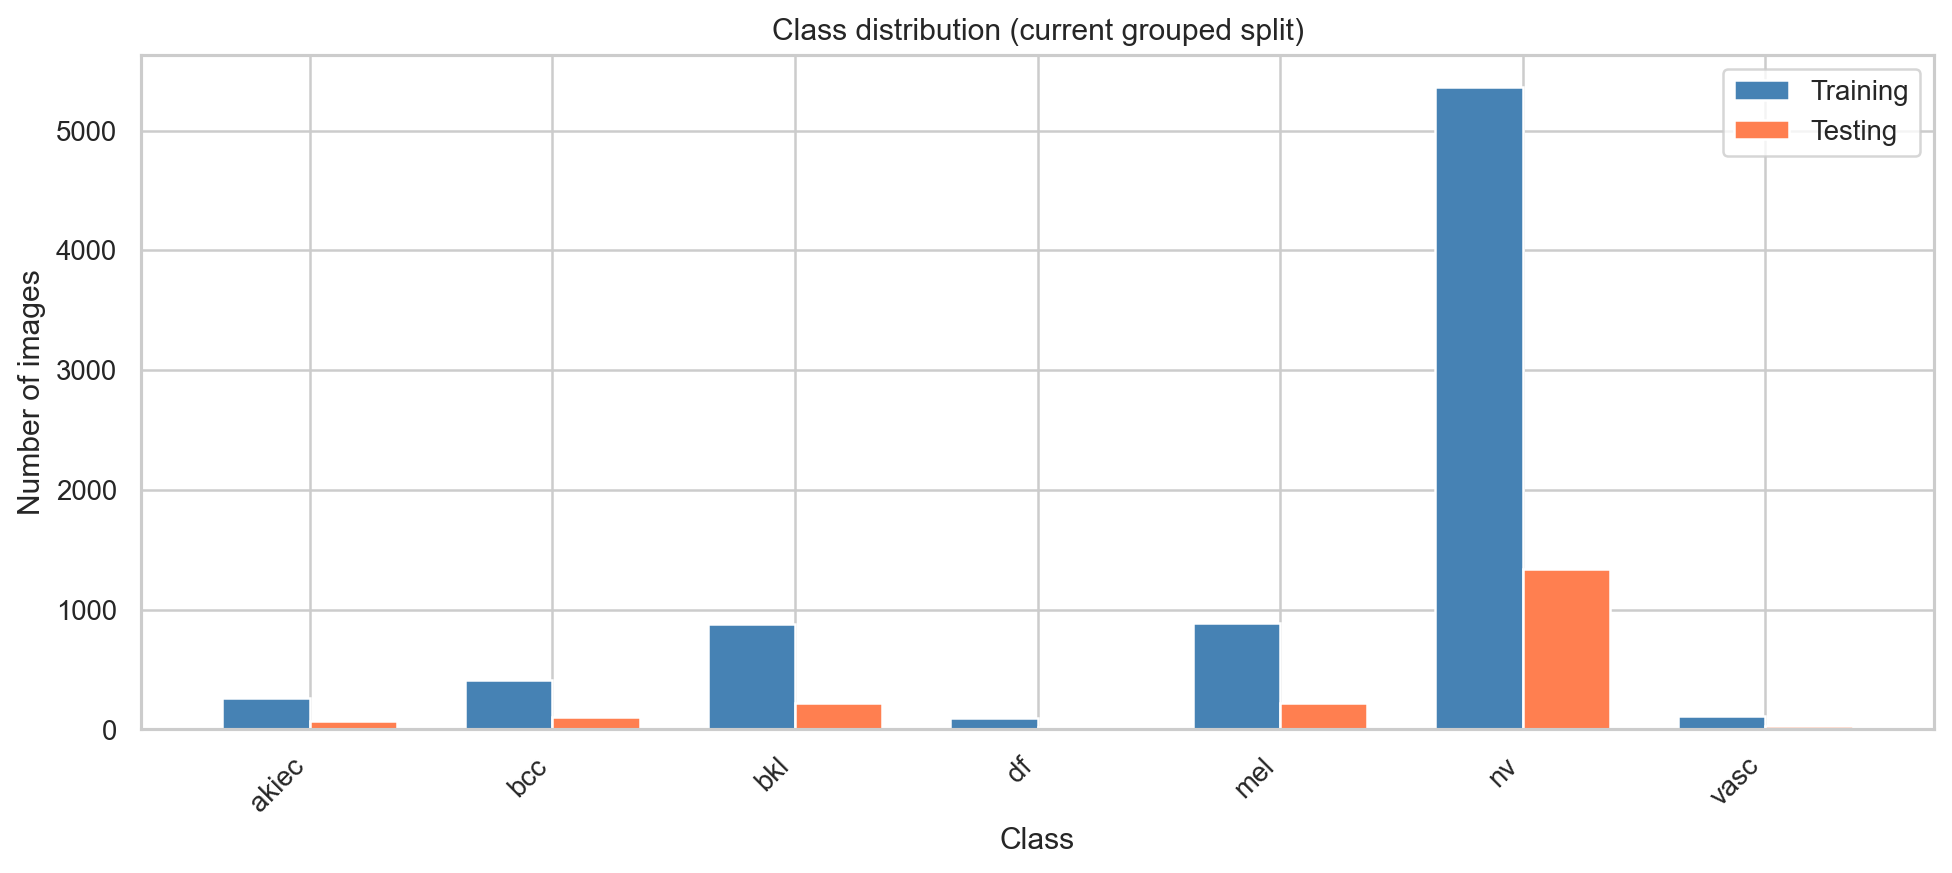
\includegraphics[width=0.84\textwidth]{class_distribution.png}
    \caption{Class distribution in the grouped split.}
    \label{fig:classdist}
\end{figure}

\begin{figure}[H]
    \centering
    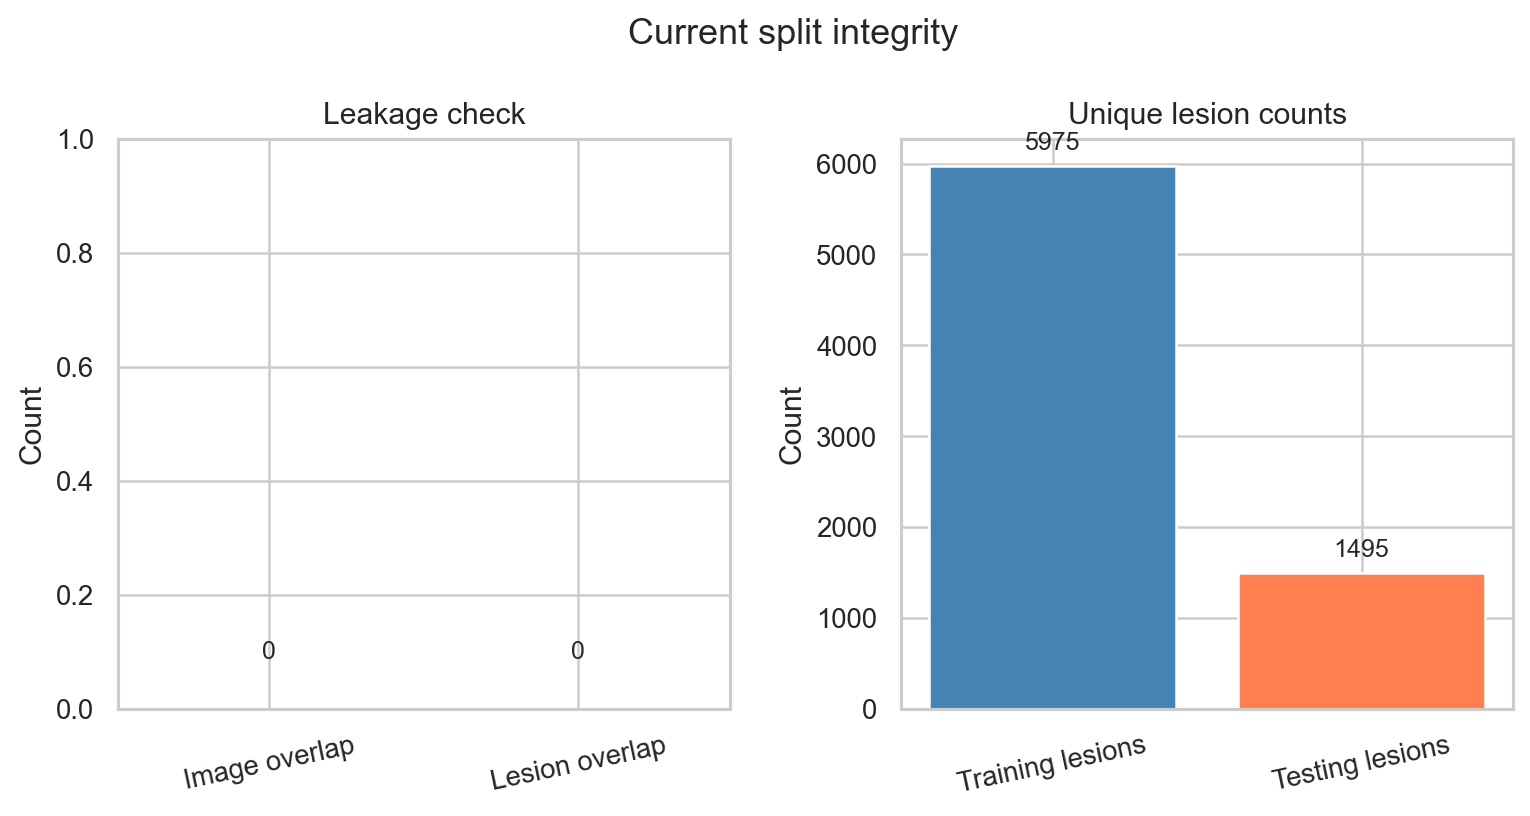
\includegraphics[width=0.80\textwidth]{split_integrity.png}
    \caption{Grouped split integrity check.}
    \label{fig:splitintegrity}
\end{figure}

Figure~\ref{fig:gallery} shows representative examples from the seven categories. Several classes overlap in color, border quality, and internal texture, which helps explain why per-class evaluation remains necessary even when overall accuracy is high.

\begin{figure}[H]
    \centering
    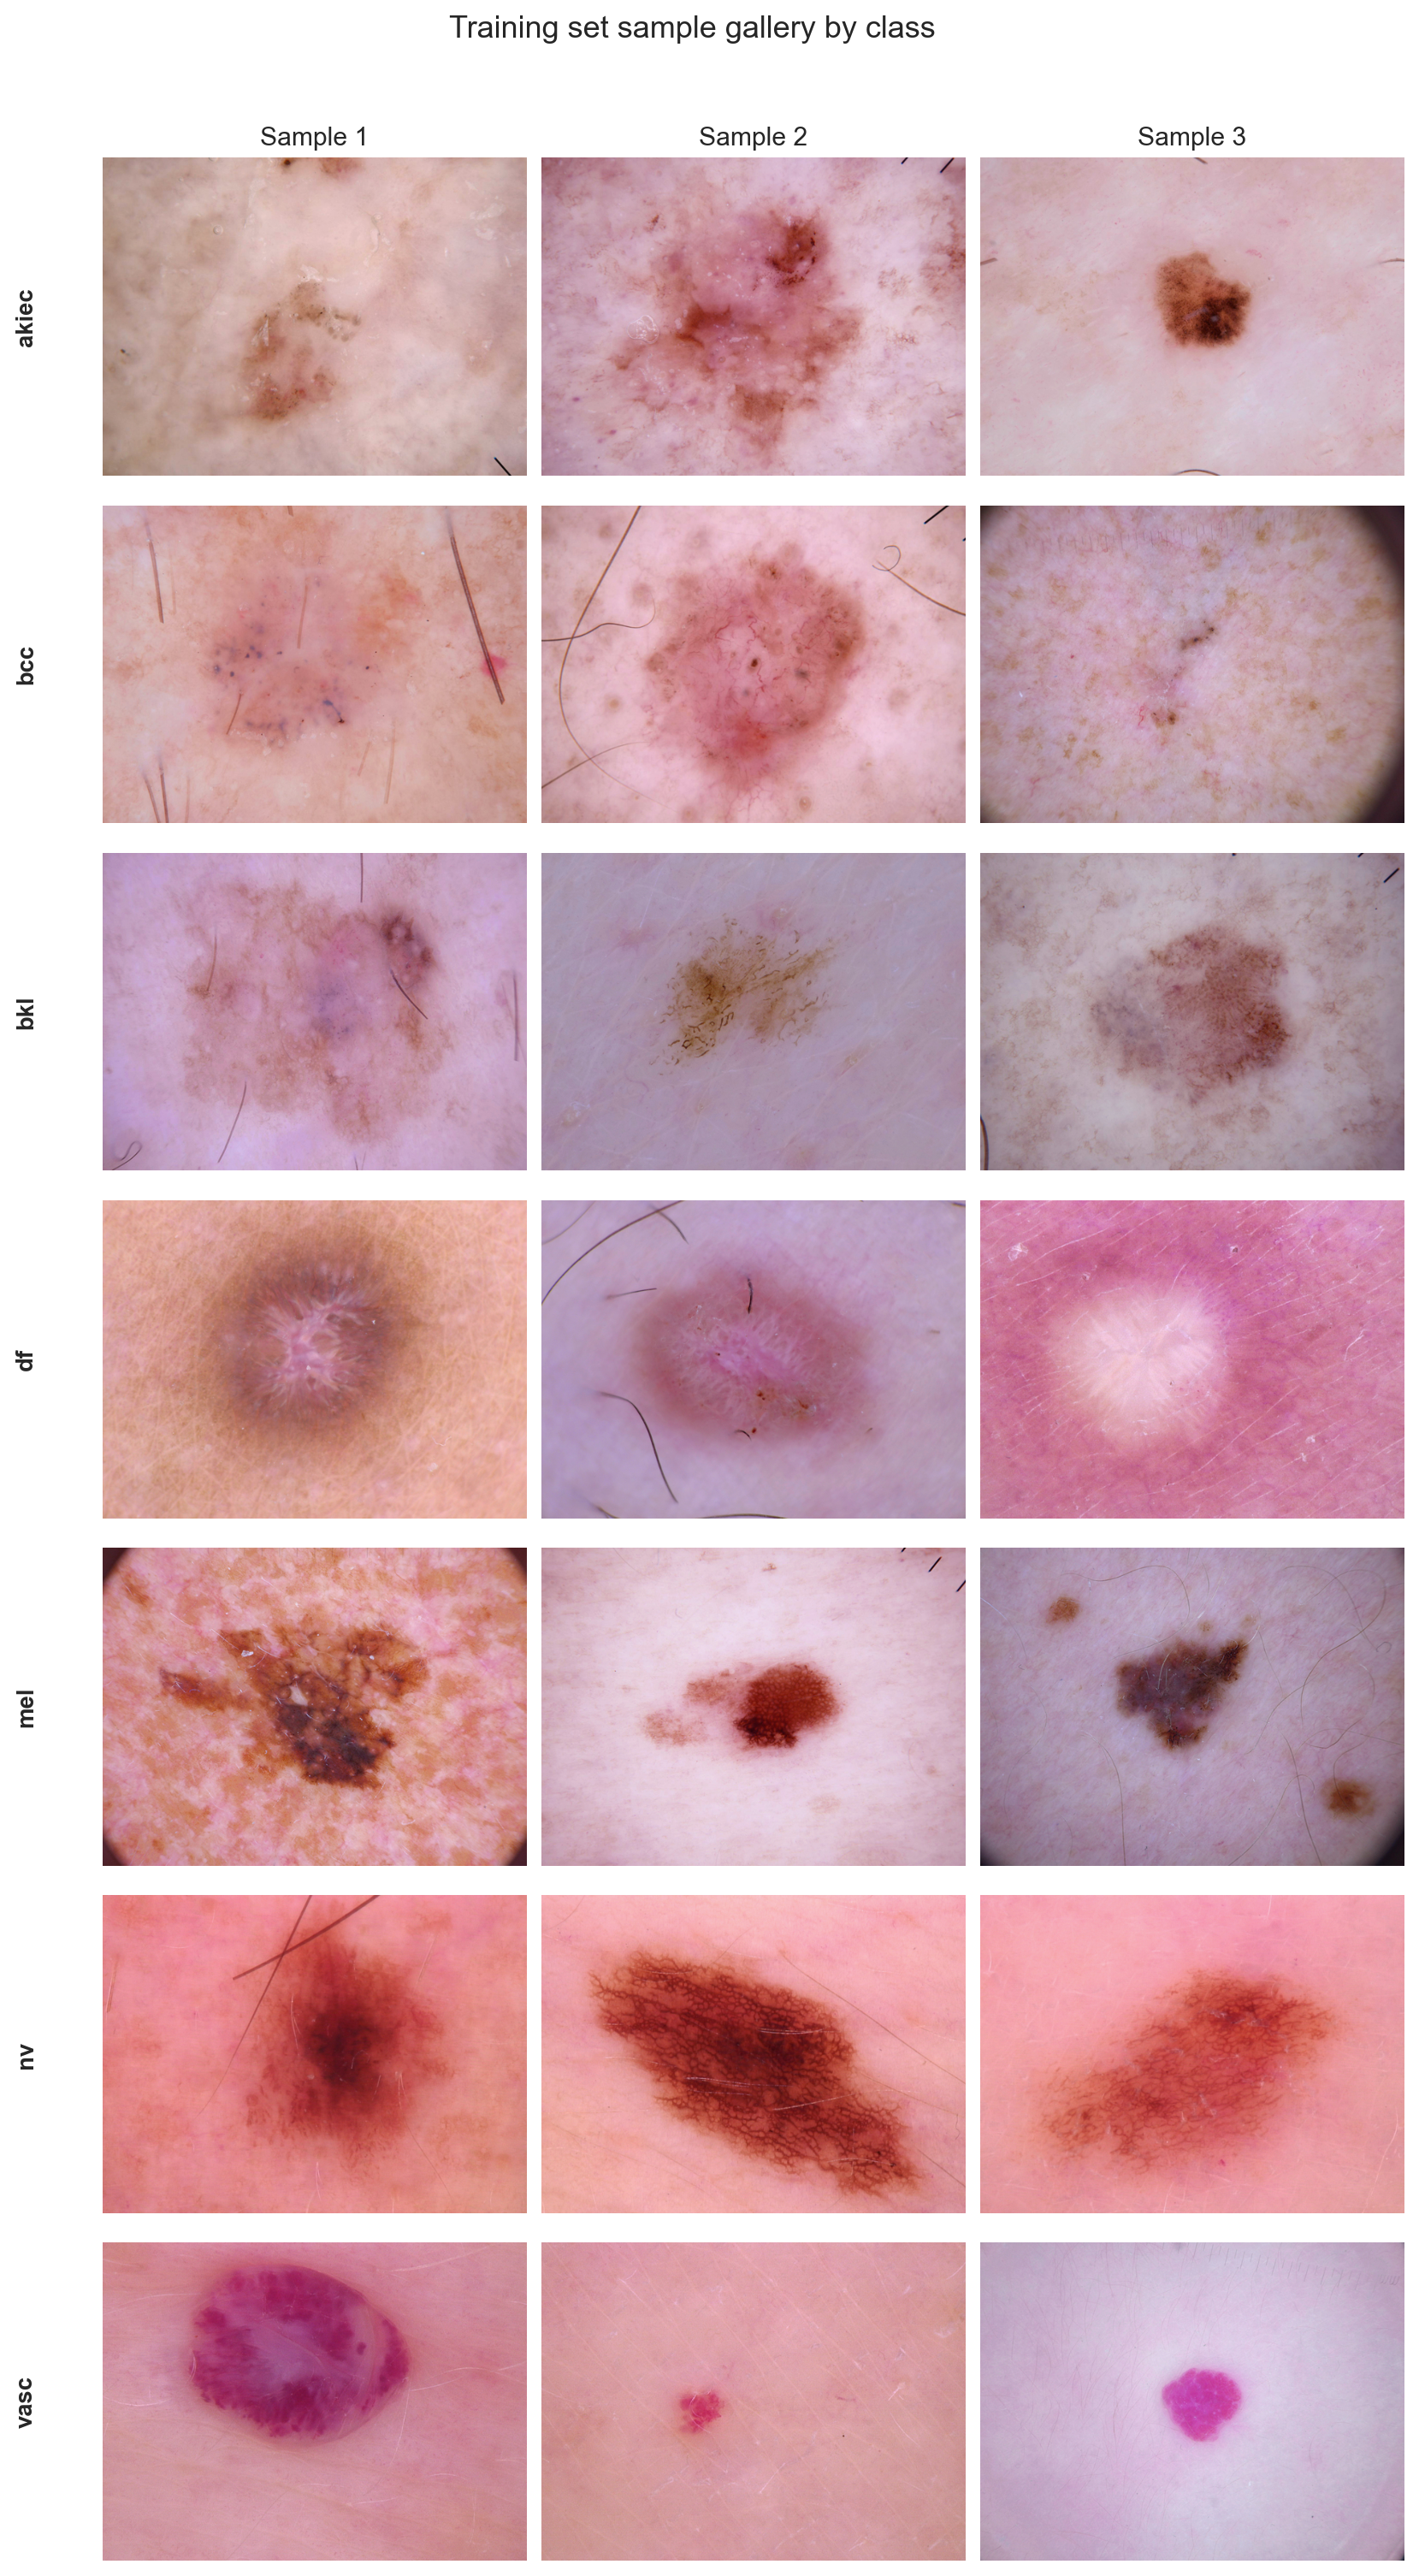
\includegraphics[width=0.70\textwidth]{sample_gallery.png}
    \caption{Representative training examples from the seven classes.}
    \label{fig:gallery}
\end{figure}

\section{Evaluation Metrics and Experimental Setup}

The evaluation protocol follows the current repository state. The model is evaluated on the grouped test set of 2{,}004 images. Reported metrics include accuracy, macro and weighted precision/recall/F1, class-wise scores, a normalized confusion matrix, and one-vs-rest ROC and precision--recall curves.

The main settings are summarized in Table~\ref{tab:setup}. All images are resized to \(224\times224\). Training uses random flips, rotation, and color jitter, while testing and deployment use deterministic resize and normalization. The classifier is optimized with cross-entropy loss and Adam. During live inference, the backend returns the maximum softmax score and applies a confidence threshold of 0.5.

\begin{table}[H]
    \centering
    \caption{Key implementation and evaluation settings.}
    \label{tab:setup}
    \begin{tabular}{ll}
        \toprule
        Item & Current setting \\
        \midrule
        Task & Seven-class skin lesion classification \\
        Backbone & ResNet18 with SE-style channel attention \\
        Input size & \(224\times224\) RGB \\
        Training augmentation & Flip, rotation, color jitter \\
        Normalization & ImageNet mean and std \\
        Loss function & Cross-entropy \\
        Optimizer & Adam \\
        Learning rate & 0.001 \\
        Scheduler & Cosine annealing, minimum \(10^{-6}\) \\
        Batch size & 32 \\
        Epoch setting & 30 epochs \\
        Evaluation split & Grouped test set, 2{,}004 images \\
        Deployment threshold & Confidence \(<0.5\) marked unrecognized \\
        \bottomrule
    \end{tabular}
\end{table}

One methodological caution is necessary. The repository contains a valid current grouped split, but the provided model weight file predates the latest refreshed train and test organization. The reported numbers therefore represent the best available project snapshot on the current split rather than a fully controlled retraining run. A final version of the study should retrain and select checkpoints under the current split definition.

\section{Results and System Testing}

The current model reaches 0.92 accuracy on the grouped test set, with macro F1 of 0.87 and weighted F1 of 0.92. These scores are strong overall, but they should be read with class-wise results because the dataset is imbalanced.

\begin{table}[H]
    \centering
    \caption{Class-wise test performance on the grouped test set.}
    \label{tab:classmetrics}
    \begin{tabular}{lrrrr}
        \toprule
        Class & Precision & Recall & F1 & Support \\
        \midrule
        akiec & 0.86 & 0.82 & 0.84 & 66 \\
        bcc   & 0.90 & 0.96 & 0.93 & 103 \\
        bkl   & 0.92 & 0.83 & 0.87 & 220 \\
        df    & 0.89 & 0.74 & 0.81 & 23 \\
        mel   & 0.82 & 0.71 & 0.76 & 222 \\
        nv    & 0.94 & 0.98 & 0.96 & 1{,}341 \\
        vasc  & 1.00 & 0.86 & 0.93 & 29 \\
        \bottomrule
    \end{tabular}
\end{table}

Figure~\ref{fig:confusion} and Figure~\ref{fig:perclass} show the same pattern from two views. Performance is strongest on the large nevus class, while melanoma remains the most difficult category and is still confused with nevus in a noticeable fraction of cases.

\begin{figure}[H]
    \centering
    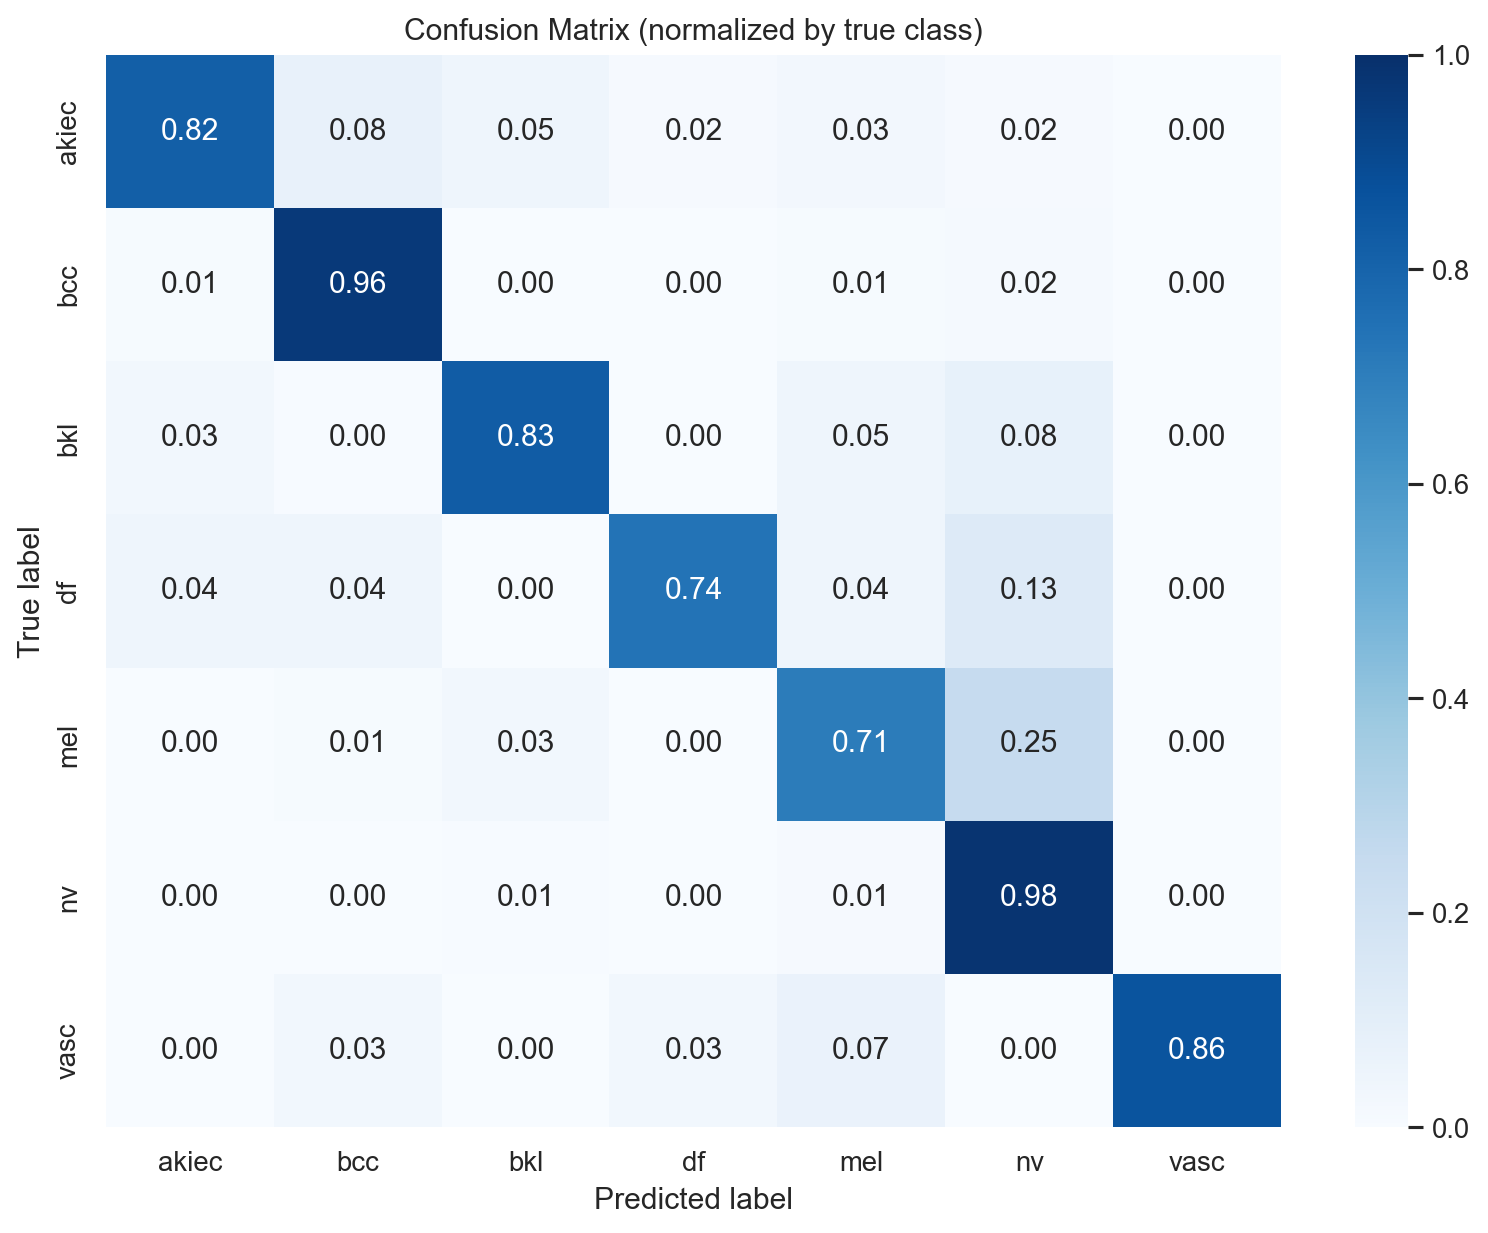
\includegraphics[width=0.80\textwidth]{confusion_matrix_normalized.png}
    \caption{Normalized confusion matrix on the grouped test set.}
    \label{fig:confusion}
\end{figure}

\begin{figure}[H]
    \centering
    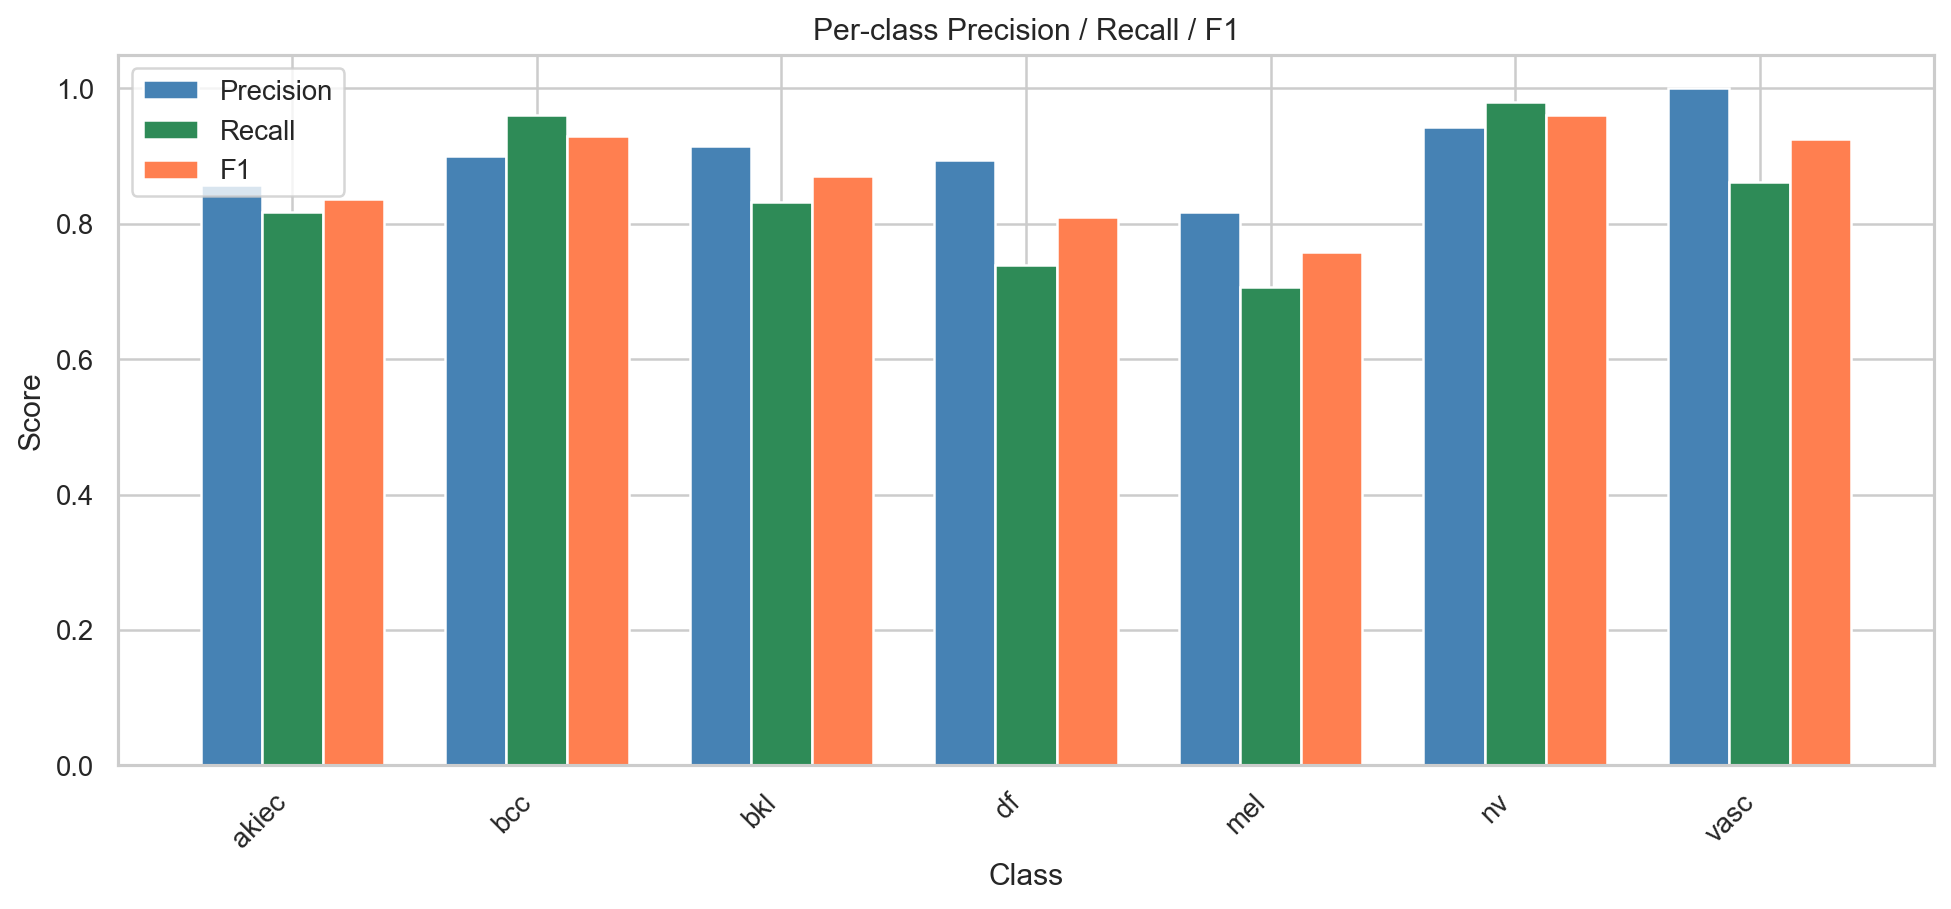
\includegraphics[width=0.86\textwidth]{per_class_metrics.png}
    \caption{Per-class precision, recall, and F1.}
    \label{fig:perclass}
\end{figure}

The ROC and precision--recall curves provide a threshold-independent view of the same results. ROC curves remain strong across classes, while the precision--recall curves make the class imbalance more visible and show that \texttt{mel} is the least stable class as recall increases.

\begin{figure}[H]
    \centering
    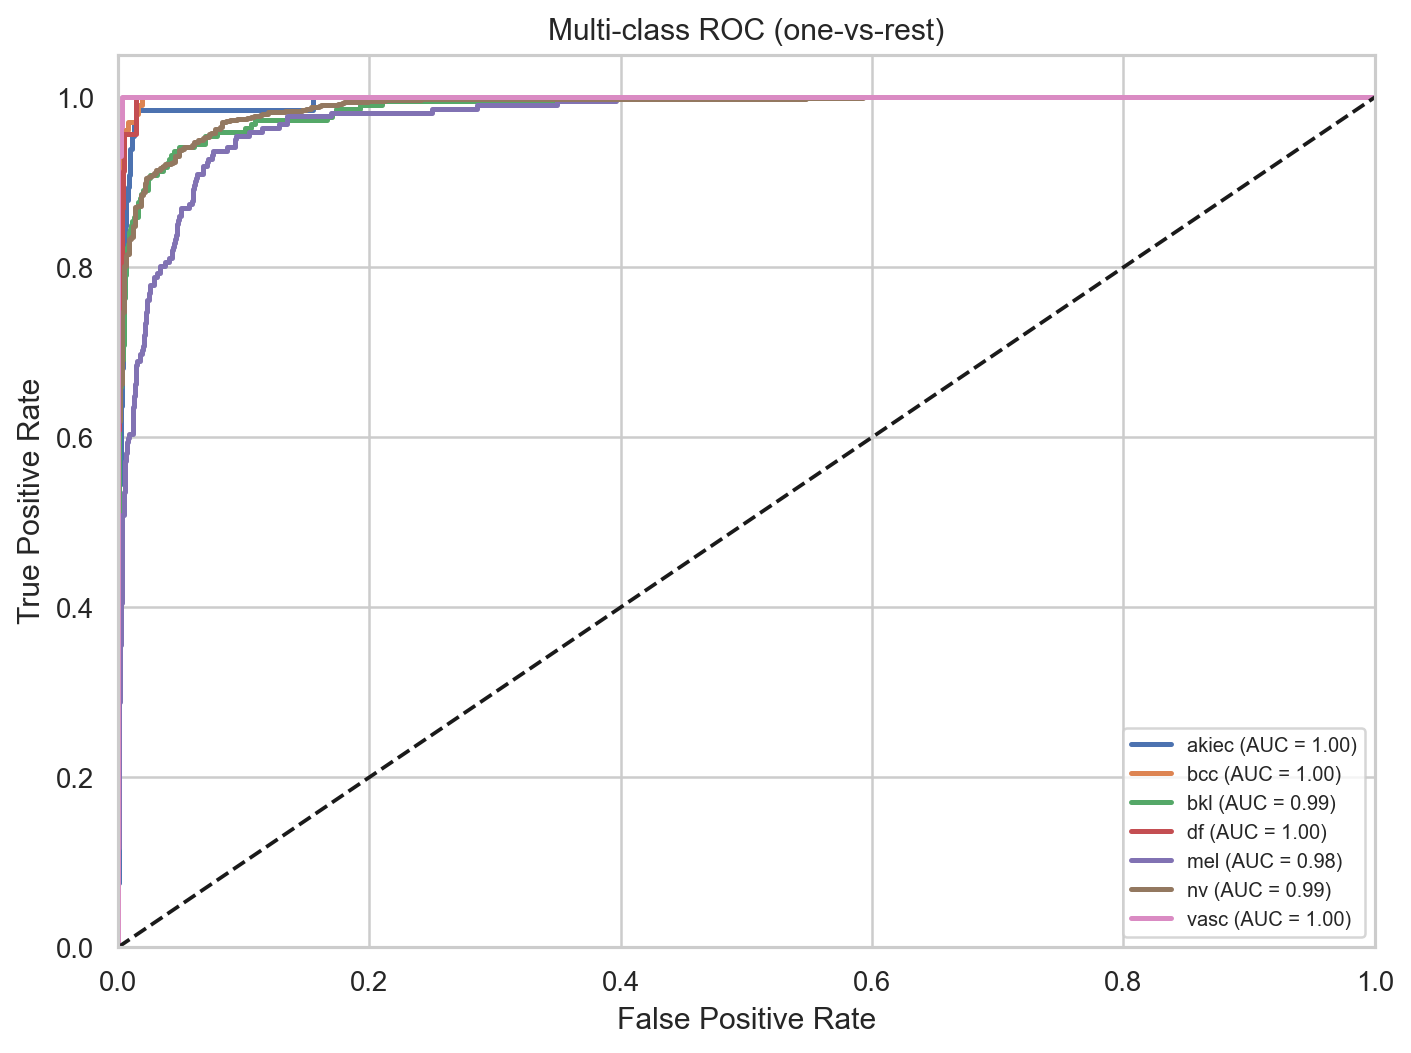
\includegraphics[width=0.86\textwidth]{roc_curves.png}
    \caption{One-vs-rest ROC curves on the grouped test set.}
    \label{fig:roc}
\end{figure}

\begin{figure}[H]
    \centering
    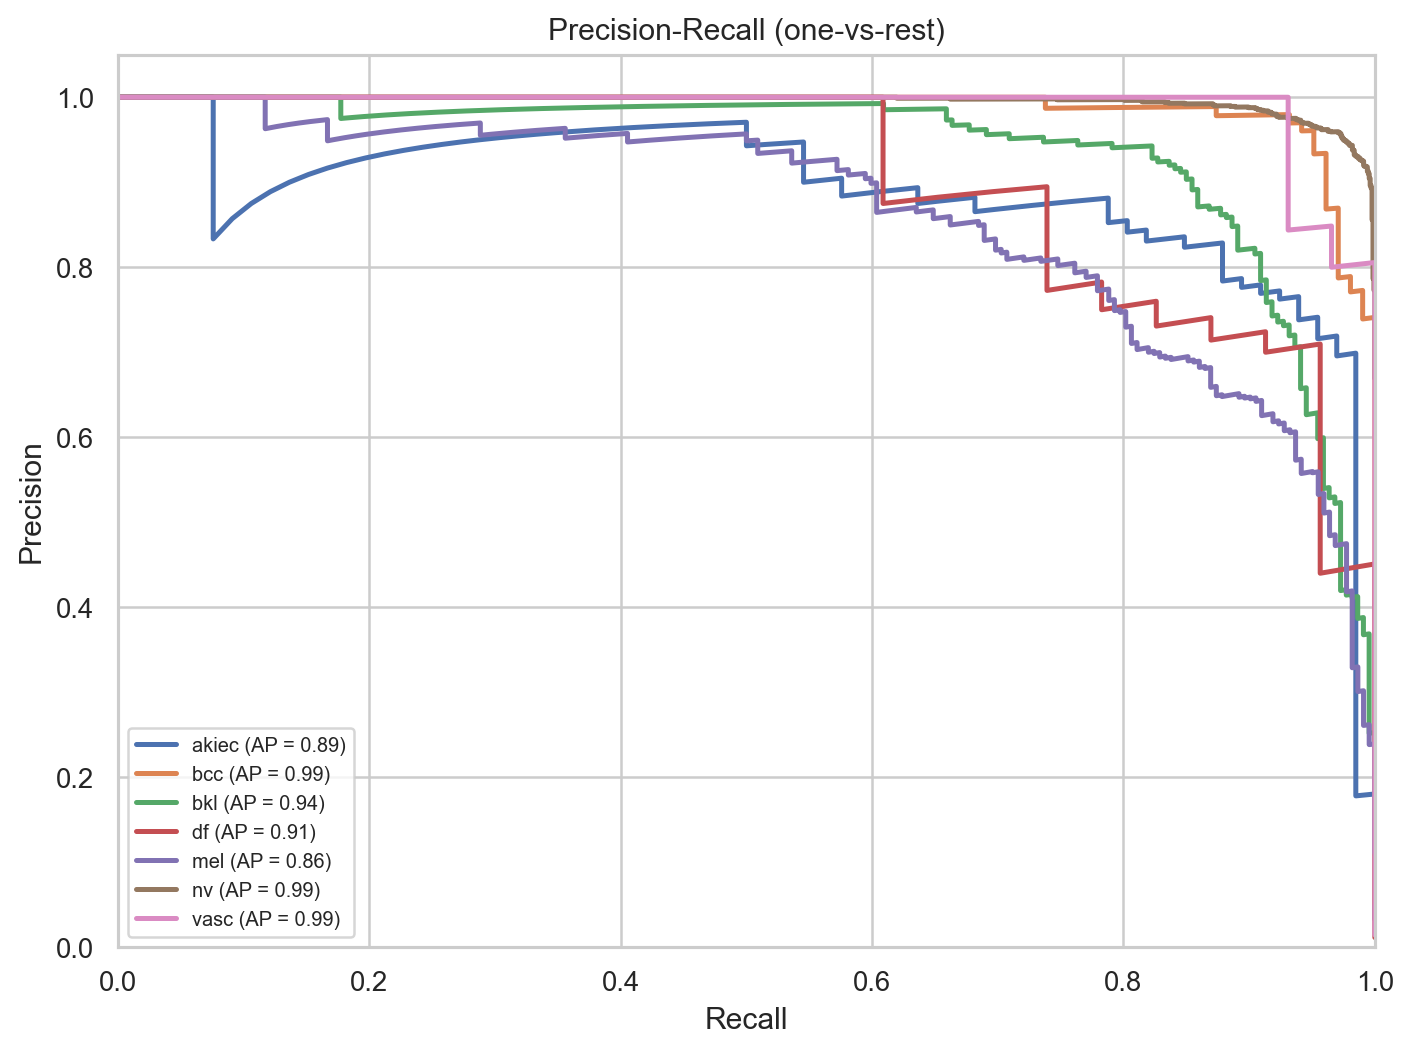
\includegraphics[width=0.86\textwidth]{pr_curves.png}
    \caption{One-vs-rest precision--recall curves.}
    \label{fig:pr}
\end{figure}

Figure~\ref{fig:ui} shows the current front-end interface. In local checks, the service loaded the model correctly, returned a normal response from \texttt{/health}, and completed a full prediction request with stored history.

\begin{figure}[H]
    \centering
    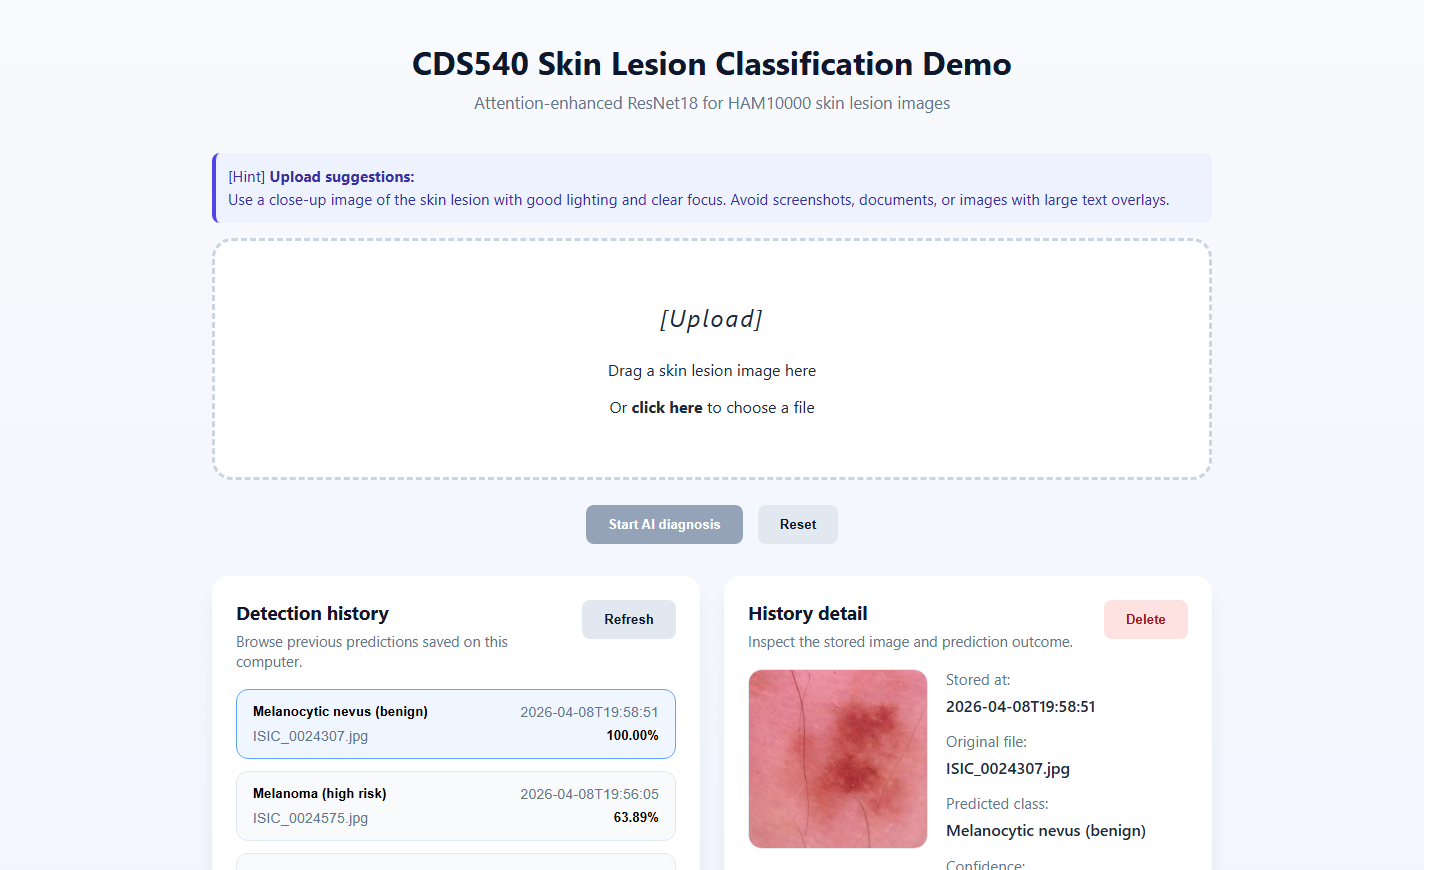
\includegraphics[width=0.92\textwidth]{ui_home_cropped.png}
    \caption{Current front-end interface served by FastAPI.}
    \label{fig:ui}
\end{figure}

\section{Discussion}

The project has several clear strengths. It uses a real public dermoscopic dataset, removes the most obvious train--test leakage problem by grouping on lesion identifiers, and connects the classifier to a usable front end. The ResNet18 backbone and attention block also provide a practical balance between standard image classification design and local deployment.

The main limitations are also clear. First, class imbalance remains substantial, and the gap in recall shows that not all diagnostic categories are treated equally. Second, the training workflow does not maintain a separate validation loop, which weakens model selection and makes older validation-style figures unusable for the current project state.

Another limitation concerns result traceability. The current grouped split is cleaner than the older image-level split, but the provided weight file appears older than the latest regenerated data folders. The model should therefore be retrained on the exact current split before stronger empirical claims are made.

Deployment logic also remains simple. The blank-image filter is a color heuristic rather than a learned out-of-distribution detector, the confidence threshold is not calibrated, and the interface does not yet provide richer audit features such as saved heatmaps or batch upload.

\section{Conclusion and Future Work}

This project presents a complete local pipeline for skin lesion image classification built around HAM10000, a ResNet18-based classifier with channel attention, and a browser-accessible FastAPI interface. The current implementation organizes the data into a grouped train--test split, applies standard preprocessing and augmentation, evaluates the model with class-aware metrics, and exposes the predictor through a lightweight web service. The best available project snapshot reaches 0.92 accuracy on the current grouped test set and supports stable local inference with prediction history.

The project is valuable because it connects dataset preparation, model design, evaluation, and deployment in one coherent workflow. The same inspection also makes the next steps clear.

Future work should focus on three related areas. First, the training pipeline needs a dedicated validation stage and a retraining run on the current grouped split so that checkpoint selection, reported metrics, and prepared data remain aligned. Better handling of class imbalance would also help the smallest classes and melanoma.

Second, the system can be extended without changing its overall design. Useful additions include batch upload, filtered history browsing, exported prediction logs, clearer error handling, simple visual explanations, and stronger experiment tracking with saved training curves and checkpoint metadata.


\bibliographystyle{plainnat}
\bibliography{references}

\end{document}
